
\documentclass{ppgeesa}

%%%%%%%%%%%%%%%%%%%%%%%%%%%%%%%%%%%%%%%%%%%%%%%%%%%%%%%%%%%%%%%%%%%%%%%%%%%%%%%%%%%%%%%%%%%%%%%%%%%%%%%%%%%%%%%%%

\usepackage[latin1]{inputenc}
\usepackage{graphicx}
\usepackage{hyperref}
\usepackage{tikz}
\usepackage{amsmath}
\usepackage{listings}
\makeatletter
\def\@xobeysp{ }
\makeatother

\lstset{ %
language=Matlab,                % choose the language of the code
basicstyle=\footnotesize,       % the size of the fonts that are used for the code
numbers=none,                   % where to put the line-numbers
numberstyle=\footnotesize,      % the size of the fonts that are used for the line-numbers
stepnumber=2,                   % the step between two line-numbers. If it's 1 each line 
                                % will be numbered
numbersep=5pt,                  % how far the line-numbers are from the code
backgroundcolor=\color{white},  % choose the background color. You must add \usepackage{color}
showspaces=false,               % show spaces adding particular underscores
showstringspaces=false,         % underline spaces within strings
showtabs=false,                 % show tabs within strings adding particular underscores
frame=false,	                % adds a frame around the code
tabsize=2,		                % sets default tabsize to 2 spaces
captionpos=b,                   % sets the caption-position to bottom
breaklines=true,                % sets automatic line breaking
breakatwhitespace=true,         % sets if automatic breaks should only happen at whitespace
title=\lstname,                 % show the filename of files included with \lstinputlisting;
                                % also try caption instead of title
escapeinside={\%*}{*)}         % if you want to add a comment within your code
%morekeywords={*,...}            % if you want to add more keywords to the set
}
\lstset{caption=Descriptive Caption Text,label=DescriptiveLabel}

% reference : http://en.wikibooks.org/wiki/LaTeX/Hyperlinks
\hypersetup{
    bookmarks=true,												% show bookmarks bar?
    unicode=false,												% non-Latin characters in Acrobat�s bookmarks
    pdftoolbar=true,											% show Acrobat�s toolbar?
    pdfmenubar=true,											% show Acrobat�s menu?
    pdffitwindow=false,											% window fit to page when opened
    pdfstartview={FitH},										% fits the width of the page to the window
    pdftitle={Modelagem e identifica��o de sistemas},			% title
    pdfauthor={Tassiano Neuhausi (tassianors@gmail.com)},		% author
    pdfsubject={M�todos param�tricos de identifica��o de sistemas},   % subject of the document
    pdfcreator={Tassiano Neuhaus},								% creator of the document
    pdfproducer={Producer},										% producer of the document
    pdfkeywords={Identifica��o de sistemas} {M�todos param�tricos}, % list of keywords
    pdfnewwindow=true,											% links in new window
    colorlinks=true,											% false: boxed links; true: colored links
    linkcolor=black,											% color of internal links
    citecolor=red,												% color of links to bibliography
    filecolor=magenta,											% color of file links
    urlcolor=blue												% color of external links
}

%%%%%%%%%%%%%%%%%%%%%%%%%%%%%%%%%%%%%%%%%%%%%%%%%%%%%%%%%%%%%%%%%%%%%%%%%%%%%%%%%%%%%%%%%%%%%%%%%%%%%%%%%%%%%%%%%


\begin{document}

\title{Modelagem e Identifica��o de sistemas lineares}

\author{Tassiano Neuhaus\\
{\small Universidade Federal do Rio Grande do Sul - Departamento de Engenharia El�trica\\Av. Osvaldo Aranha, 103 - Bairro Bom Fim CEP: 90035-190 - Porto Alegre - RS - Brasil}\\
}%\thanks{Tassiano Neuhaus, tassianors@gmail.com, tel +55-51-91760154}

\maketitle

\thispagestyle{empty}\pagestyle{empty}

\begin{abstract}
%===============================================================================
% ABSTRACT
%===============================================================================

Neste trabalho ser� apresentado diversos meios para a identifica��o de sistemas
lineares. Existem dois grupos principais de m�todos para esta identifica��o, sendo
um deles conhecido como {\it{identifica��o n�o param�trica}} onde existem infinitos
par�metros para serem estimados e que normalmente � utilizado para identifica��o de
fun��es gr�ficas. Outro m�todo � conhecido como {\it{identifica��o param�trica}} onde
o n�mero de par�metros a ser estimado � finito. Este �ltimo m�todo ser� mais abordado
neste trabalho, por possuir uma aplicabilidade maior devido a possibilidade de estimar 
processos em fun��es matem�ticas que descrevem o comportamento do sistema muitas vezes
com mais informa��o que os m�todos gr�ficos.

Para este trabalho ser� utilizado um processo de controle de posi��o angular, controlado
por um motor de corrente continua. Ser�o apresentados diversos m�todos de identifica��o 
e ao fim ser� feito um comparativo entre os resultados obtidos.


\end{abstract}

\begin{IEEEkeywords}
Identifica��o de sistemas lineares, m�todos param�tricos.
\end{IEEEkeywords}

%===============================================================================
\section{Introdu��o}

Neste trabalho ser� apresentado o projeto de controladores denominados Robustos. Para 
tanto ser� apresentado o conceito de um controlador Robusto. A fim de modelar um
sistema sujeito a incertezas ser� apresentado alguns m�todos para que sua modelagem
matem�tica seja poss�vel. 

Para tornar o estudo mais claro ser� utilizado um sistema f�sico onde estar� sujeito a
perturba��es e/ou incertezas. Sobre este sistema ser� feito a modelagem seguindo cada um
dos processos e com estes modelos ser� efetuado uma simula��o. 

Esta simula��o ser� baseada no projeto de uma realimenta��o de estados com o intuito de
satisfazer a minimiza��o da norma $H2$ e $H_{\infty}$.

O sistema utilizado � apresentado no sistema de equa��es de estado descrito em (\ref{eq:intro_sis}).

\begin{equation}
\begin{matrix}
A=\begin{bmatrix}
0 & 1\\ 
-ba &a+b 
\end{bmatrix} &
B=\begin{bmatrix}
0\\ 
k
\end{bmatrix} 
\end{matrix}
\label{eq:intro_sis}
\end{equation}

Este sistema possui a fun��o de transfer�ncia apresentado em (\ref{eq:intro_transf}).

\begin{equation}
G(s)=\frac{k}{(s-a)(s-b)}
\label{eq:intro_transf}
\end{equation}

Os par�metros $a, b, k$ est�o sujeitos as varia��es apresentadas em (\ref{eq:intro_limit}).

\begin{equation}
\begin{matrix}
b= & -0.012725 & \\ 
k= & [k_1 \; k_2] =& [-0.4649.10^{-4} \; -0.7449.10^{-4}]\\ 
a= & [a_1 \; a_2] =& [-0.25 \; -2]
\end{matrix}
\label{eq:intro_limit}
\end{equation}


\section{Modelagem do sistema}
\label{sec:modelling}
%===============================================================================

O objetivo da modelagem de um sistema � encontrar um modelo (fun��o com par�metros
livres) que consiga representar o sistema f�sico de forma completa. A partir do
conhecimento do sistema f�sico, fazem-se considera��es sobre o sistema, para simplifica-lo
a fim de tornar o modelo matem�tico o mais simples poss�vel, mas que ainda represente
o sistema real, com a margem de preciosidade definida, pela quantidade e qualidade 
das simplifica��es aplicadas para chegar-se ao modelo matem�tico do sistema.

\subsection{Sistema F�sico}
%===============================================================================

O sistema f�sico em estudo neste trabalho, � um sistema para controle de posi��o, onde 
o atuador � um motor de corrente continua (DC). Desta forma a entrada do sistema 
� a tens�o aplicada sobre os terminais do motor em Volts [V], e a sa�da � a posi��o
angular do motor em radianos [rad].

Na Figura (\ref{fig:motor_system}) pode ser vista a representa��o el�trica e mec�nica
do motor em quest�o.

\begin{figure}[htbp]
	\center
	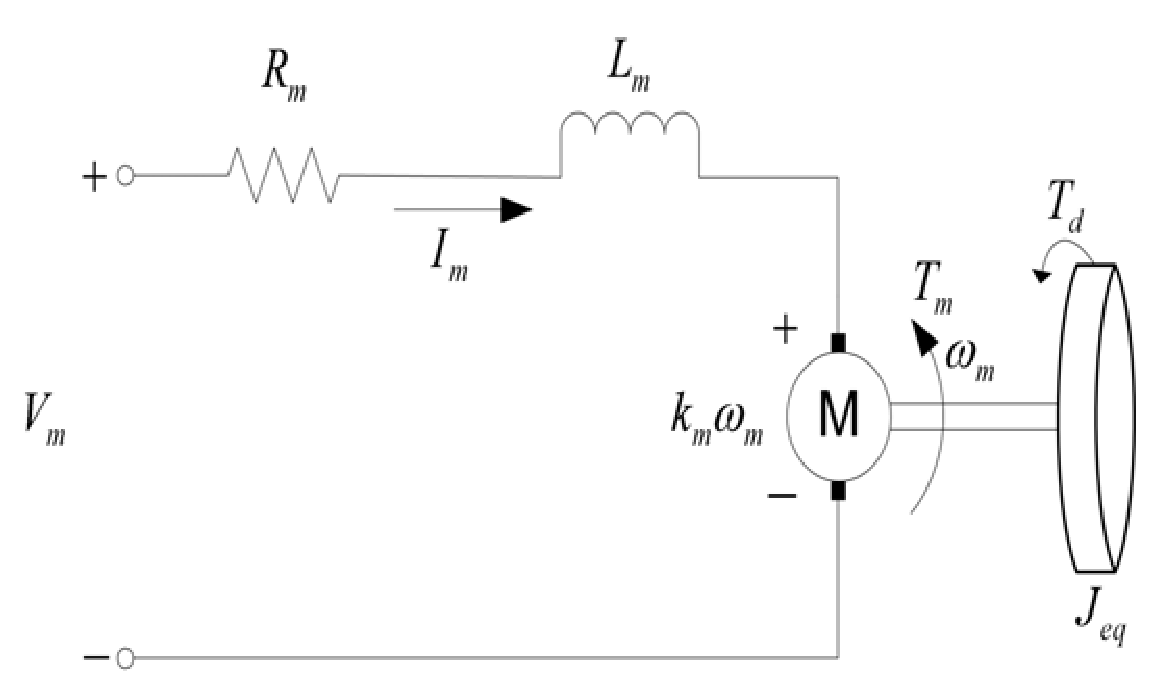
\includegraphics[width=0.7\columnwidth]{figures/motor_system.eps}
	\caption{Representa��o el�trica e mec�nica do motor}
	\label{fig:motor_system}
\end{figure}

As vari�veis consideradas para a modelagem s�o as apresentadas abaixo:

\begin{itemize}
	\item $\omega$ = Velocidade do motor.
	\item \it{v} = Tens�o aplicada na armadura.
	\item \it{ia} = corrente de armadura.
	\item \it{L} = Indut�ncia da armadura.
	\item \it{e} = Forca contra eletromotriz = $K_{2} \omega$
	\item \it{R} = Resist�ncia do enrolamento da armadura.
	\item \it{T} = Torque aplicado = $K_{i} ia$
	\item \it{J} = Momento de inercia da carga.
	\item \it{f} = Atrito viscoso no eixo.
\end{itemize}

Tem-se desta forma as duas equac�es que descrevem o sistema para a parte el�trica
(\ref{eq:motor_elet}) e mec�nica (\ref{eq:motor_mec}).

\begin{equation}
V-R\cdot Ia - L\frac{\mathrm{d} Ia}{\mathrm{d} x}-e = 0
\label{eq:motor_elet}
\end{equation}

\begin{equation}
J \dot{\omega}= T-f\omega
\label{eq:motor_mec}
\end{equation}

A partir destas equac�es diferenciais pode-se chegar ao sistema de equac�es de estado 
descrito em (\ref{eq:motor_eq_estados}).

\begin{equation}
\begin{matrix}
\begin{bmatrix}
\dot{Ia}\\ 
\dot{\omega} \\
\dot{\theta}
\end{bmatrix}= &
\begin{bmatrix}
-R/L & -K_2/L & 0\\ 
K_i/J & -f/J & 0 \\
0 & 1 & 0
\end{bmatrix}&
\begin{bmatrix}
Ia\\ 
\omega \\
\theta
\end{bmatrix} + &
\begin{bmatrix}
1\\ 
0\\
0
\end{bmatrix} V
\end{matrix}
\label{eq:motor_eq_estados}
\end{equation}

Com este sistema de equac�es de estado, � poss�vel obter-se as fun�es de transfer�ncias,
que descrevem o sistema, para uma entrada e uma sa�da. Na equac�o (\ref{eq:motor_pos_tf}) 
apresenta-se a func�o de transferencia do motor, que relaciona a posic�o com a tens�o de entrada
do motor.

\begin{equation}
G(s)=\frac{k1/JL}{s(s+f/L)(s+R/L)+s\;k1 k2/JL}
\label{eq:motor_pos_tf}
\end{equation}

Devido a dinamica do sistema mecanico ser muito menor que a dinamica do sistema el�trico, 
pode-se desconsiderar a influencia do polo el�trico do sistema, ficando a func�o de transfereicia
como a seguir:

\begin{equation}
G(s)=\frac{\frac{k1}{JL}}{s(s+\frac{fL+k1 k2}{JL})}
\label{eq:motor_pos_tf}
\end{equation}


\section{Modelagem n�o param�trica}
\label{sec:non_parametric}
%===============================================================================




\section{Modelos param�tricos simples}
\label{sec:parametric}
%===============================================================================



\section{M�todo dos m�nimos quadrados}
\label{sec:mmq}
%===============================================================================

O m�todo dos m�nimos quadrados (MMQ) � um dos mais conhecidos e mais utilizados 
nas mais diversas �reas da ci�ncia e tecnologia. A origem da ideia b�sica pode ser
encontrada nos trabalhos de Gaus sobre o estudo astron�micos. \cite{aguirre}

\subsection{Sistema com solu��o �nica}
%===============================================================================

Considerando-se que o sistema que ser� observado seja linear e invariante no tempo.
Se a fun��o $f$ que descreve o sistema for n�o linear o sistema poder� em principio 
ser identificado por modelos n�o lineares. Com base nestas restri��es temos que:

\begin{equation}
\begin{matrix}
\begin{matrix}
\begin{bmatrix}
y_1\\ 
y_2\\ 
\vdots \\ 
y_n
\end{bmatrix} = &
\begin{bmatrix}
x_1 & x_2 & \cdots  & x_n
\end{bmatrix} &
\begin{bmatrix}
\theta_1\\ 
\theta_2\\ 
\vdots \\ 
\theta_n
\end{bmatrix}
\end{matrix}
\\ \\
y=X\theta
\end{matrix}
\nonumber
\end{equation}

Com $X \in \Re^{nxn}$. Desde que $X$ seja n�o singular � poss�vel determinar $\theta$:

\begin{equation}
\theta=X^{-1}y
\label{eq:mmq_base}
\end{equation}

\subsection{Sistema sobredeterminado}
%===============================================================================

Para sistemas sobredeterminados onde $ N > n$, A vari�vel $X$ da equa��o (\ref{eq:mmq_base}) fica
$X \in \Re^{Nxn}$. Como esta matriz n�o � quadrada, n�o � poss�vel de ser invertida. Multiplicando-se
a equa��o (\ref{eq:mmq_base}) por $X^T$ tem-se: \cite{aguirre}

\begin{equation}
X^Ty=X^TX\theta
\nonumber
\end{equation}

De onde vem:

\begin{equation}
\theta = [X^T X]^{-1} X^T y
\label{eq:mmq}
\end{equation}

O m�todo dos m�nimos quadrados minimiza o crit�rio apresentado em (\ref{eq:mmq_j}).

\begin{equation}
J(\theta)=\frac{1}{2N}\sum_{t=1}^{N}[y(t)-\hat{y}(t, \theta)]^2
\label{eq:mmq_j}
\end{equation}

Onde $\hat{y}(t, \theta)$ � a predi��o do sistema e pode ser representado como abaixo:

\begin{equation}
\hat{y}(t, \theta)=\theta^T \phi(t)
\nonumber
\end{equation}

Desta forma pode se dizer que o sistema real � o pr�prio sistema estimado mais algum 
erro de estimativa:

\begin{equation}
y(t) = \hat{y}(t, \theta) +e(t)=\theta^T \phi(t) + e(t)
\nonumber
\end{equation}

\subsection{Estruturas de modelagem}
%===============================================================================

De forma gen�rica modelos para descri��o de sistemas podem ser representados como em 
(\ref{eq:mmq_generic_model}).

\begin{equation}
A(q, \theta)Y(t)=\frac{B(q, \theta)}{F(q, \theta)}U(t)+\frac{C(q, \theta)}{D(q, \theta)}e(t)
\label{eq:mmq_generic_model}
\end{equation}

Onde:

\begin{equation}
\begin{matrix}
A(q, \theta)=1+a_1 q^{-1}+a_2 q^{-2}+\cdots +a_{na} q^{-na}\\
B(q, \theta)=b_1 q^{-1}+b_2 q^{-2}+\cdots +b_{nb} q^{-nb}\\ 
C(q, \theta)=1+c_1 q^{-1}+c_2 q^{-2}+\cdots +c_{nc} q^{-nc}\\ 
D(q, \theta)=1+d_1 q^{-1}+d_2 q^{-2}+\cdots +d_{na} q^{-nd}\\ 
F(q, \theta)=1+f_1 q^{-1}+f_2 q^{-2}+\cdots +f_{nf} q^{-nf} 
\end{matrix}
\nonumber
\end{equation}

Baseado nestas informa��es existem modelos onde apenas alguns destes polin�mios s�o 
diferentes de 1. Na Tabela (\ref{tab:model}) s�o apresentados alguns destes modelos
mais comumente utilizados.

\begin{table}[htbp]
  \begin{center}
	\caption{Modelos comumente utilizados para identifica��o de sistemas}
	\label{tab:model}
	\begin{small}
	  \begin{tabular}{rc}
		\hline
		Modelo & Polin�mios diferentes de 1 \\
		\hline
		FIR	& B \\
		ARX	& A B \\
		ARMAX & A B C \\
		ARMA & A C \\
		ARARMAX & A B C D \\
		OE & B F \\
		BJ & B F C D \\
		\hline
	  \end{tabular}
	\end{small}
  \end{center}
\end{table}

O m�todo dos m�nimos quadrados utiliza intrinsecamente o modelo ARX para descrever 
o modelo do sistema.

\subsection{Controle de posi��o angular do motor DC}
%===============================================================================

O sistema descrito na se��o (\ref{sec:modelling}) quando utilizamos o m�todo dos 
m�nimos quadrados, intrinsecamente utilizamos o modelo ARX (\ref{eq:mmq_arx}) para 
descrever este sistema. A partir de (\ref{eq:mmq_generic_model}) tem-se que o
modelo ARX fica (\ref{eq:mmq_arx}).

\begin{equation}
A(q, \theta)Y(t)=B(q, \theta)U(t)+e(t)
\label{eq:mmq_arx}
\end{equation}

A equa��o (\ref{eq:mmq_arx}) pode ser reescrita :

\begin{equation}
\begin{matrix}
Y(t)=b_1 q^{-1}U(t)+b_2 q^{-2}U(t)+\cdots +b_{nb} q^{-nb}U(t)\\
	 -a_1 q^{-1}Y(t)-b_2 q^{-2}Y(t)-\cdots -a_{na} q^{-na}Y(t) + e(t)
\end{matrix}
\nonumber
\end{equation}

O que pode ser escrito como em (\ref{eq:mmq_yt}).

\begin{equation}
Y(t)=\varphi ' \theta +e(t)
\label{eq:mmq_yt}
\end{equation}

Onde:

\begin{equation}
\begin{matrix}
\theta = \begin{bmatrix}
a_1\\ 
\vdots \\ 
a_{na}\\ 
b_1\\ 
\vdots \\ 
b_{nb}
\end{bmatrix}
 & 
\varphi (t)=\begin{bmatrix}
y(t-1)\\ 
\vdots \\ 
y(t-na)\\ 
u(t-1)\\ 
\vdots \\ 
u(t-nb)
\end{bmatrix}
\\ 
& \\
\Phi = \begin{bmatrix}
\varphi '(1)\\ 
\varphi '(2)\\ 
\vdots\\ 
\varphi '(N)
\end{bmatrix} & 
\end{matrix}
\nonumber
\end{equation}

Para o sistema de posicionamento do motor DC, a equa��o (\ref{eq:mmq_arx})
fica como em (\ref{eq:mmq_motor_arx}).

\begin{equation}
G(q, \theta)=\frac{a}{(q-b)(q-c)} \;\;H(q, \theta)=\frac{q^2}{(q-b)(q-c)}
\label{eq:mmq_motor_arx}
\end{equation}

A partir de (\ref{eq:mmq_motor_arx}) tem-se que o modelo pode ser descrito como 
abaixo:

\begin{equation}
\begin{matrix}
\theta = \begin{bmatrix}
a & b+c & c
\end{bmatrix}
&
\varphi (t)=\begin{bmatrix}
r(t-2)\\ 
y(t-1)\\ 
y(t-2)
\end{bmatrix}
\end{matrix}
\nonumber
\end{equation}

Sabe-se de antem�o que o valor esperado para a vari�vel $c$ � zero, j� que existe um 
integrador na planta em estudo. No Ap�ndice (\ref{appendix_mmq}) est� o script utilizado 
para chegar-se aos resultados obtidos para a estimativa do modelo utilizando o m�todo dos
m�nimos quadrados.

A figura (\ref{fig:mmq_arx}) apresenta os resultados obtidos na estimativa dos par�metros
a partir das medidas efetuadas sobre o sistema.

\begin{figure}[htbp]
	\center
	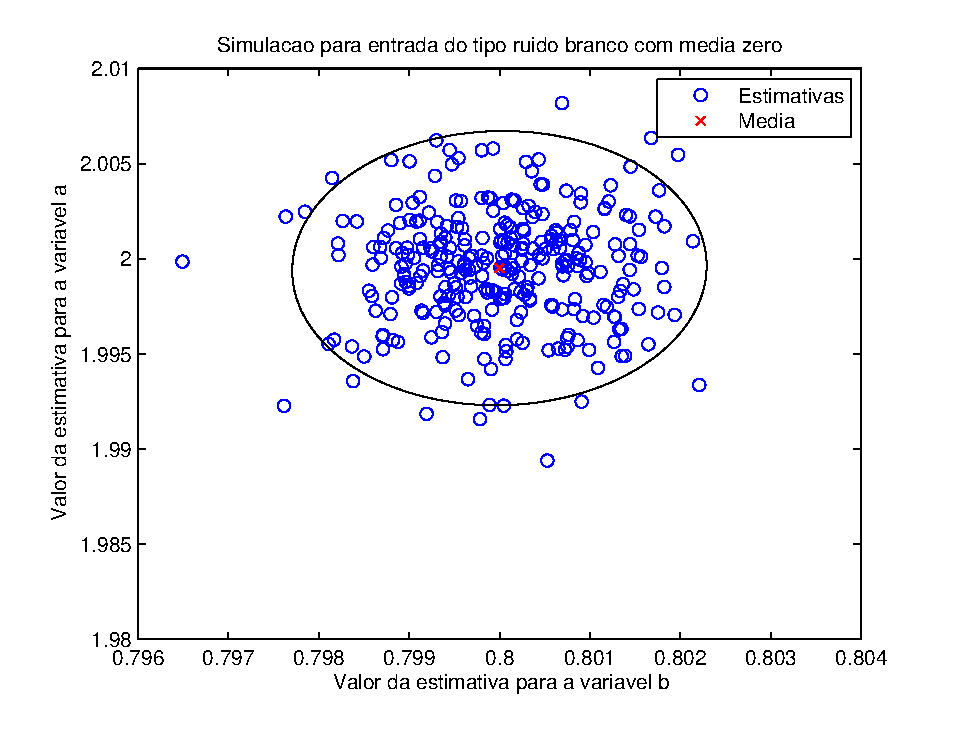
\includegraphics[width=0.98\columnwidth]{figures/mmq_arx.eps}
	\caption{TODO}
	\label{fig:mmq_arx}
\end{figure}

TODO: colocar os valores m�dios obtidos para os par�metros.

\subsubsection{Resultados para um modelo incompleto}
%===============================================================================

Nesta se��o ser� apresentado resultados para uma estimativa utilizando um modelo que n�o consegue
descrever o sistema propriamente. Ser�o utilizados os mesmos dados da estimativa do item anterior.

O modelo utilizado � descrito em (\ref{eq:mmq_motor_arx_inc}). Observa-se que o integrador n�o esta presente
neste modelo, desta forma tem-se que o modelo das vari�veis a serem utilizadas no m�todo dos 
m�nimos quadrados fica como em (\ref{eq:mmq_arx_inc_var}).

\begin{equation}
G(q, \theta)=\frac{a}{(q-b)} \;\;H(q, \theta)=\frac{q}{(q-b)}
\label{eq:mmq_motor_arx_inc}
\end{equation}

\begin{equation}
\begin{matrix}
\theta = \begin{bmatrix}
a & b 
\end{bmatrix}
&
\varphi (t)=\begin{bmatrix}
r(t-1)\\ 
y(t-1) 
\end{bmatrix}
\end{matrix}
\label{eq:mmq_arx_inc_var}
\end{equation}

Para este modelo chegou-se aos valores dos par�metros $a$ e $b$ apresentados na 
Figura (\ref{fig:mmq_arx_inc}).

\begin{figure}[htbp]
	\center
	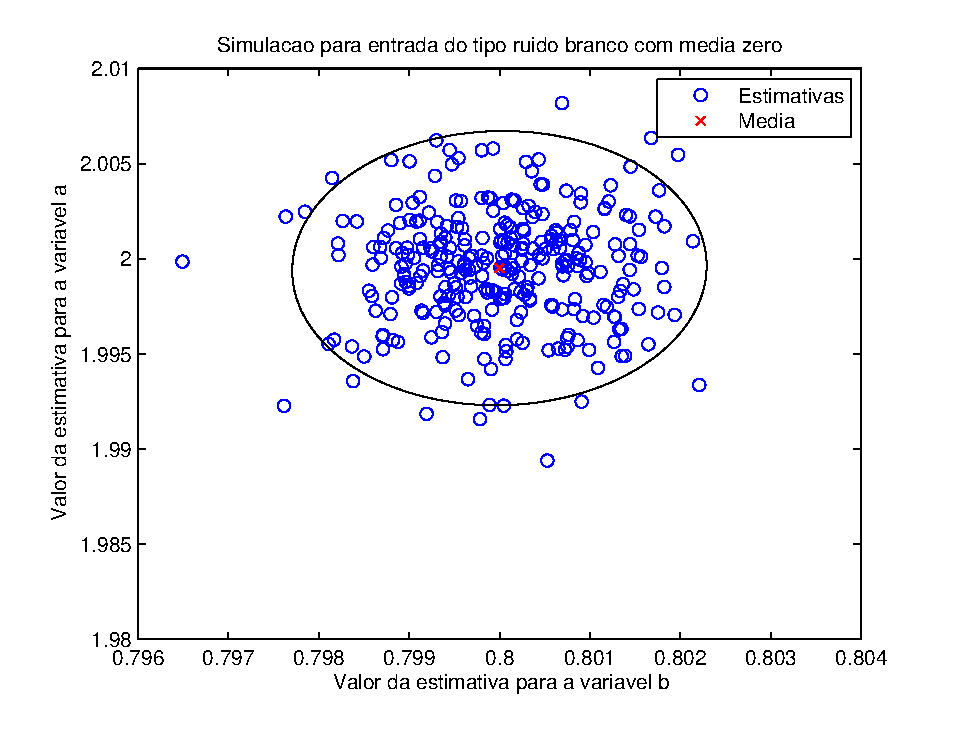
\includegraphics[width=0.98\columnwidth]{figures/mmq_arx.eps}
	\caption{TODO}
	\label{fig:mmq_arx_inc}
\end{figure}


\section{Classes de modelos Gen�ricas}
\label{sec:non_arx}
%===============================================================================



%===============================================================================
\section{Conclus�es}
\label{sec:concl}
%===============================================================================

Neste trabalho foram apresentados dois m�todos para identifica��o de sistemas lineares,
ambos os m�todos se encontram na categoria de m�todos param�tricos de identifica��o, que 
de forma simplificada, tentam estimar os par�metros de uma fun��o de transfer�ncia que
represente o sistema f�sico em quest�o. Os m�todos utilizados foram o dos m�nimos quadrados
e das vari�veis instrumentais.

O sistema f�sico utilizado foi o controle de posi��o de um motor DC, e os dados coletados
para a identifica��o foram gerados a partir da aplica��o de sinais de refer�ncia tais como
rampas, senoides e ondas quadradas. Para cada um destes conjuntos foi obtido uma estimativa
dos par�metros do modelo utilizado.

Para efetuar a estimativa do sistema f�sico em quest�o, foi necess�rio determinar um modelo,
este foi determinado baseado no conhecimento das caracter�sticas do sistema e algumas simplifica��es 
foram efetuadas, a fim de tornar o modelo matem�tico o mais simples poss�vel, mas que ainda 
consiga descrever o sistema dentro de uma margem aceit�vel de precis�o.

O m�todo dos m�nimos quadrados (\ref{sec:mmq}) obteve resultados para a estimativa dos par�metros
que podem ser encontrados na Tabela (\ref{tab:mmq_results}). Houveram pequenas diverg�ncias nos 
par�metros entre um conjunto de dados e outro, o que n�o � desej�vel, isso pode ser devido a
imprecis�es do modelo utilizado, (pode ser devido as simplifica��es do modelo, ou de din�micas n�o
levadas em considera��o).

O m�todo das vari�veis instrumentais (\ref{sec:iv}) obteve resultados semelhantes ao m�todo 
dos m�nimos quadrados, mas com valores mais pr�ximos nos diferentes grupos de medidas. Os 
resultados para este m�todo foram apresentados na Tabela (\ref{tab:iv_results}).

De forma geral este trabalho abordou e demonstrou como � o procedimento e no que se baseiam 
dois m�todos de identifica��o de sistemas lineares sujeitos a incertezas, perturba��es e 
ru�dos. N�o � o objetivo deste trabalho detalhar esmiu�ar a matem�tica destes m�todos e
sim apresentar um exemplo pr�tico, e demonstrar sua utilidade.

A aplicabilidade deste t�pico de engenharia � de uma aplicabilidade imensa, sendo muito importante 
nas mais diversas �reas a correta identifica��o de sistemas para que, a partir do conhecimento 
matem�tico de sua din�mica, possa se agir sobre este sistema, a fim de obter os resultados desejados
de forma eficiente e com propriedade sobre as a��es tomadas, uma vez que o sistema identificado
� identificado e sabe-se o qu�o boa esta aproxima��o do sistema real pode ser.

%===============================================================================
\appendix
%===============================================================================
\chapter{1 - Script para Simula��o do MQ para o modelo ARX} 
\label{appendix_mmq}
\lstset{caption=M�todo dos m�nimos quadrados,label=DescriptiveLabel}
\lstinputlisting{matlab_files/simul.m}

%===============================================================================
\chapter{2 - Script para Simula��o do m�todo das vari�veis instrumentais} 
\label{appendix_iv}
\lstset{caption=M�todo das vari�veis instrumentais,label=DescriptiveLabel}
\lstinputlisting{matlab_files/simul_iv.m}

%===============================================================================



\bibliographystyle{IEEEtran}
\bibliography{biblio}

\end{document}
